\documentclass{amsart}
\usepackage[hmargin=1.5cm,vmargin=1.65cm]{geometry}
\usepackage{tikz}
\parskip = 0.2 cm
\parindent = 0 cm

\usepackage{fancyvrb}

\begin{document}

\title{Notes on Turing machines}
\author{Eric Martin}
\address{COMP9021 Principles of Programming}
\date{Session 1, 2017}

\maketitle
\thispagestyle{empty}

\section{Division by 2 program}

\begin{verbatim}
del1 1 del2 0 R
del2 1 mov1R 0 R
mov1R 1 mov1R 1 R
mov1R 0 mov2R 0 R
mov2R 1 mov2R 1 R
mov2R 0 mov1L 1 L
mov1L 1 mov1L 1 L
mov1L 0 mov2L 0 L
mov2L 1 mov2L 1 L
mov2L 0 del1 0 R
\end{verbatim}

\section{Computation of 5 // 2}

\begin{center}
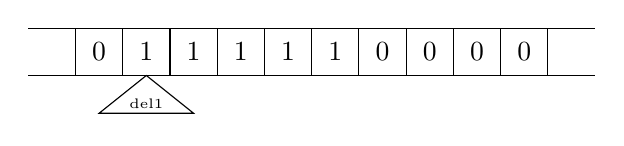
\begin{tikzpicture}[scale=0.6]
	\draw (0,0) -- (12,0);
	\draw (0,1) -- (12,1);
	\draw (1.5,0.5) node{0};
	\draw (2.5,0.5) node{1};
	\draw (3.5,0.5) node{1};
	\draw (4.5,0.5) node{1};
	\draw (5.5,0.5) node{1};
	\draw (6.5,0.5) node{1};
	\draw (7.5,0.5) node{0};
	\draw (8.5,0.5) node{0};
	\draw (9.5,0.5) node{0};
	\draw (10.5,0.5) node{0};
	\foreach \x in {1,...,11} \draw (\x,0) -- (\x,1);
	\draw (1.5, -0.8) -- (2.5, 0) -- (3.5, -0.8) -- cycle;
	\draw (2.5, -0.6) node{\tiny del1};
\end{tikzpicture}
\end{center}

\begin{center}
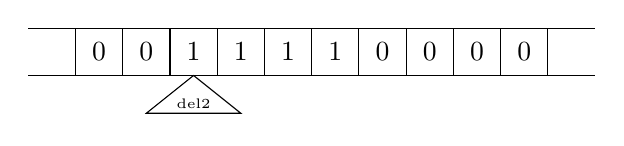
\begin{tikzpicture}[scale=0.6]
	\draw (0,0) -- (12,0);
	\draw (0,1) -- (12,1);
	\draw (1.5,0.5) node{0};
	\draw (2.5,0.5) node{0};
	\draw (3.5,0.5) node{1};
	\draw (4.5,0.5) node{1};
	\draw (5.5,0.5) node{1};
	\draw (6.5,0.5) node{1};
	\draw (7.5,0.5) node{0};
	\draw (8.5,0.5) node{0};
	\draw (9.5,0.5) node{0};
	\draw (10.5,0.5) node{0};
	\foreach \x in {1,...,11} \draw (\x,0) -- (\x,1);
	\draw (2.5, -0.8) -- (3.5, 0) -- (4.5, -0.8) -- cycle;
	\draw (3.5, -0.6) node{\tiny del2};
\end{tikzpicture}
\end{center}

\begin{center}
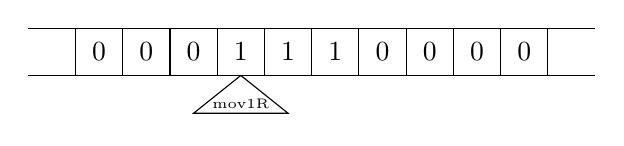
\begin{tikzpicture}[scale=0.6]
	\draw (0,0) -- (12,0);
	\draw (0,1) -- (12,1);
	\draw (1.5,0.5) node{0};
	\draw (2.5,0.5) node{0};
	\draw (3.5,0.5) node{0};
	\draw (4.5,0.5) node{1};
	\draw (5.5,0.5) node{1};
	\draw (6.5,0.5) node{1};
	\draw (7.5,0.5) node{0};
	\draw (8.5,0.5) node{0};
	\draw (9.5,0.5) node{0};
	\draw (10.5,0.5) node{0};
	\foreach \x in {1,...,11} \draw (\x,0) -- (\x,1);
	\draw (3.5, -0.8) -- (4.5, 0) -- (5.5, -0.8) -- cycle;
	\draw (4.5, -0.6) node{\tiny mov1R};
\end{tikzpicture}
\end{center}

\begin{center}
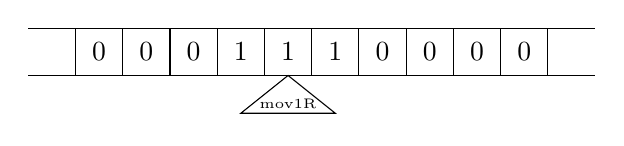
\begin{tikzpicture}[scale=0.6]
	\draw (0,0) -- (12,0);
	\draw (0,1) -- (12,1);
	\draw (1.5,0.5) node{0};
	\draw (2.5,0.5) node{0};
	\draw (3.5,0.5) node{0};
	\draw (4.5,0.5) node{1};
	\draw (5.5,0.5) node{1};
	\draw (6.5,0.5) node{1};
	\draw (7.5,0.5) node{0};
	\draw (8.5,0.5) node{0};
	\draw (9.5,0.5) node{0};
	\draw (10.5,0.5) node{0};
	\foreach \x in {1,...,11} \draw (\x,0) -- (\x,1);
	\draw (4.5, -0.8) -- (5.5, 0) -- (6.5, -0.8) -- cycle;
	\draw (5.5, -0.6) node{\tiny mov1R};
\end{tikzpicture}
\end{center}

\begin{center}
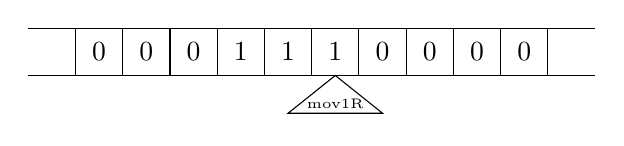
\begin{tikzpicture}[scale=0.6]
	\draw (0,0) -- (12,0);
	\draw (0,1) -- (12,1);
	\draw (1.5,0.5) node{0};
	\draw (2.5,0.5) node{0};
	\draw (3.5,0.5) node{0};
	\draw (4.5,0.5) node{1};
	\draw (5.5,0.5) node{1};
	\draw (6.5,0.5) node{1};
	\draw (7.5,0.5) node{0};
	\draw (8.5,0.5) node{0};
	\draw (9.5,0.5) node{0};
	\draw (10.5,0.5) node{0};
	\foreach \x in {1,...,11} \draw (\x,0) -- (\x,1);
	\draw (5.5, -0.8) -- (6.5, 0) -- (7.5, -0.8) -- cycle;
	\draw (6.5, -0.6) node{\tiny mov1R};
\end{tikzpicture}
\end{center}

\begin{center}
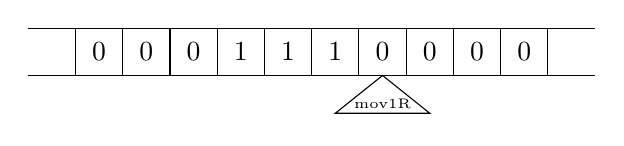
\begin{tikzpicture}[scale=0.6]
	\draw (0,0) -- (12,0);
	\draw (0,1) -- (12,1);
	\draw (1.5,0.5) node{0};
	\draw (2.5,0.5) node{0};
	\draw (3.5,0.5) node{0};
	\draw (4.5,0.5) node{1};
	\draw (5.5,0.5) node{1};
	\draw (6.5,0.5) node{1};
	\draw (7.5,0.5) node{0};
	\draw (8.5,0.5) node{0};
	\draw (9.5,0.5) node{0};
	\draw (10.5,0.5) node{0};
	\foreach \x in {1,...,11} \draw (\x,0) -- (\x,1);
	\draw (6.5, -0.8) -- (7.5, 0) -- (8.5, -0.8) -- cycle;
	\draw (7.5, -0.6) node{\tiny mov1R};
\end{tikzpicture}
\end{center}

\begin{center}
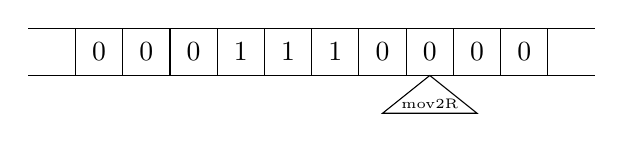
\begin{tikzpicture}[scale=0.6]
	\draw (0,0) -- (12,0);
	\draw (0,1) -- (12,1);
	\draw (1.5,0.5) node{0};
	\draw (2.5,0.5) node{0};
	\draw (3.5,0.5) node{0};
	\draw (4.5,0.5) node{1};
	\draw (5.5,0.5) node{1};
	\draw (6.5,0.5) node{1};
	\draw (7.5,0.5) node{0};
	\draw (8.5,0.5) node{0};
	\draw (9.5,0.5) node{0};
	\draw (10.5,0.5) node{0};
	\foreach \x in {1,...,11} \draw (\x,0) -- (\x,1);
	\draw (7.5, -0.8) -- (8.5, 0) -- (9.5, -0.8) -- cycle;
	\draw (8.5, -0.6) node{\tiny mov2R};
\end{tikzpicture}
\end{center}

\begin{center}
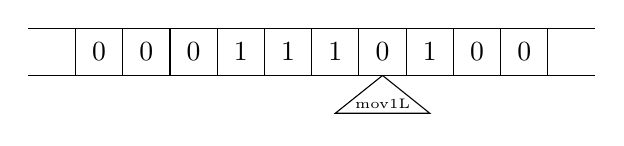
\begin{tikzpicture}[scale=0.6]
	\draw (0,0) -- (12,0);
	\draw (0,1) -- (12,1);
	\draw (1.5,0.5) node{0};
	\draw (2.5,0.5) node{0};
	\draw (3.5,0.5) node{0};
	\draw (4.5,0.5) node{1};
	\draw (5.5,0.5) node{1};
	\draw (6.5,0.5) node{1};
	\draw (7.5,0.5) node{0};
	\draw (8.5,0.5) node{1};
	\draw (9.5,0.5) node{0};
	\draw (10.5,0.5) node{0};
	\foreach \x in {1,...,11} \draw (\x,0) -- (\x,1);
	\draw (6.5, -0.8) -- (7.5, 0) -- (8.5, -0.8) -- cycle;
	\draw (7.5, -0.6) node{\tiny mov1L};
\end{tikzpicture}
\end{center}

\begin{center}
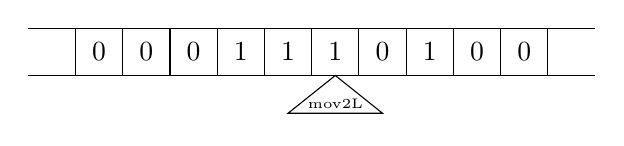
\begin{tikzpicture}[scale=0.6]
	\draw (0,0) -- (12,0);
	\draw (0,1) -- (12,1);
	\draw (1.5,0.5) node{0};
	\draw (2.5,0.5) node{0};
	\draw (3.5,0.5) node{0};
	\draw (4.5,0.5) node{1};
	\draw (5.5,0.5) node{1};
	\draw (6.5,0.5) node{1};
	\draw (7.5,0.5) node{0};
	\draw (8.5,0.5) node{1};
	\draw (9.5,0.5) node{0};
	\draw (10.5,0.5) node{0};
	\foreach \x in {1,...,11} \draw (\x,0) -- (\x,1);
	\draw (5.5, -0.8) -- (6.5, 0) -- (7.5, -0.8) -- cycle;
	\draw (6.5, -0.6) node{\tiny mov2L};
\end{tikzpicture}
\end{center}

\begin{center}
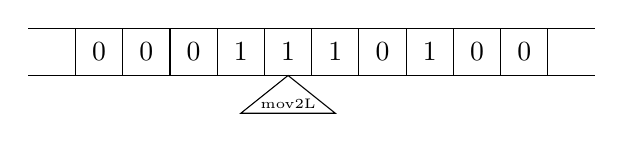
\begin{tikzpicture}[scale=0.6]
	\draw (0,0) -- (12,0);
	\draw (0,1) -- (12,1);
	\draw (1.5,0.5) node{0};
	\draw (2.5,0.5) node{0};
	\draw (3.5,0.5) node{0};
	\draw (4.5,0.5) node{1};
	\draw (5.5,0.5) node{1};
	\draw (6.5,0.5) node{1};
	\draw (7.5,0.5) node{0};
	\draw (8.5,0.5) node{1};
	\draw (9.5,0.5) node{0};
	\draw (10.5,0.5) node{0};
	\foreach \x in {1,...,11} \draw (\x,0) -- (\x,1);
	\draw (4.5, -0.8) -- (5.5, 0) -- (6.5, -0.8) -- cycle;
	\draw (5.5, -0.6) node{\tiny mov2L};
\end{tikzpicture}
\end{center}

\begin{center}
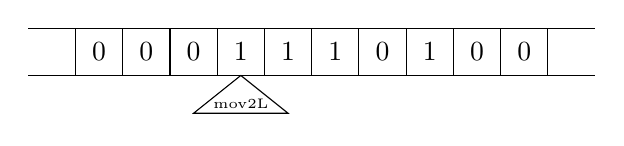
\begin{tikzpicture}[scale=0.6]
	\draw (0,0) -- (12,0);
	\draw (0,1) -- (12,1);
	\draw (1.5,0.5) node{0};
	\draw (2.5,0.5) node{0};
	\draw (3.5,0.5) node{0};
	\draw (4.5,0.5) node{1};
	\draw (5.5,0.5) node{1};
	\draw (6.5,0.5) node{1};
	\draw (7.5,0.5) node{0};
	\draw (8.5,0.5) node{1};
	\draw (9.5,0.5) node{0};
	\draw (10.5,0.5) node{0};
	\foreach \x in {1,...,11} \draw (\x,0) -- (\x,1);
	\draw (3.5, -0.8) -- (4.5, 0) -- (5.5, -0.8) -- cycle;
	\draw (4.5, -0.6) node{\tiny mov2L};
\end{tikzpicture}
\end{center}

\begin{center}
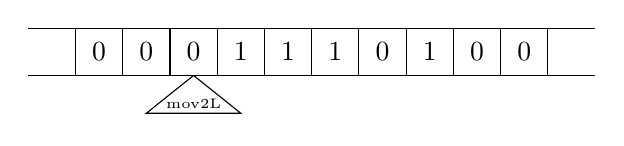
\begin{tikzpicture}[scale=0.6]
	\draw (0,0) -- (12,0);
	\draw (0,1) -- (12,1);
	\draw (1.5,0.5) node{0};
	\draw (2.5,0.5) node{0};
	\draw (3.5,0.5) node{0};
	\draw (4.5,0.5) node{1};
	\draw (5.5,0.5) node{1};
	\draw (6.5,0.5) node{1};
	\draw (7.5,0.5) node{0};
	\draw (8.5,0.5) node{1};
	\draw (9.5,0.5) node{0};
	\draw (10.5,0.5) node{0};
	\foreach \x in {1,...,11} \draw (\x,0) -- (\x,1);
	\draw (2.5, -0.8) -- (3.5, 0) -- (4.5, -0.8) -- cycle;
	\draw (3.5, -0.6) node{\tiny mov2L};
\end{tikzpicture}
\end{center}

\begin{center}
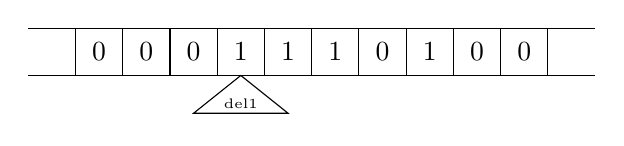
\begin{tikzpicture}[scale=0.6]
	\draw (0,0) -- (12,0);
	\draw (0,1) -- (12,1);
	\draw (1.5,0.5) node{0};
	\draw (2.5,0.5) node{0};
	\draw (3.5,0.5) node{0};
	\draw (4.5,0.5) node{1};
	\draw (5.5,0.5) node{1};
	\draw (6.5,0.5) node{1};
	\draw (7.5,0.5) node{0};
	\draw (8.5,0.5) node{1};
	\draw (9.5,0.5) node{0};
	\draw (10.5,0.5) node{0};
	\foreach \x in {1,...,11} \draw (\x,0) -- (\x,1);
	\draw (3.5, -0.8) -- (4.5, 0) -- (5.5, -0.8) -- cycle;
	\draw (4.5, -0.6) node{\tiny del1};
\end{tikzpicture}
\end{center}

\begin{center}
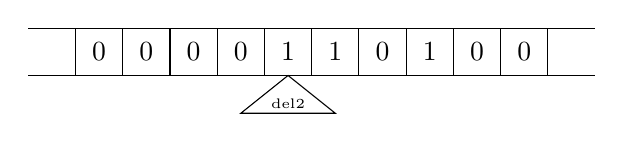
\begin{tikzpicture}[scale=0.6]
	\draw (0,0) -- (12,0);
	\draw (0,1) -- (12,1);
	\draw (1.5,0.5) node{0};
	\draw (2.5,0.5) node{0};
	\draw (3.5,0.5) node{0};
	\draw (4.5,0.5) node{0};
	\draw (5.5,0.5) node{1};
	\draw (6.5,0.5) node{1};
	\draw (7.5,0.5) node{0};
	\draw (8.5,0.5) node{1};
	\draw (9.5,0.5) node{0};
	\draw (10.5,0.5) node{0};
	\foreach \x in {1,...,11} \draw (\x,0) -- (\x,1);
	\draw (4.5, -0.8) -- (5.5, 0) -- (6.5, -0.8) -- cycle;
	\draw (5.5, -0.6) node{\tiny del2};
\end{tikzpicture}
\end{center}

\begin{center}
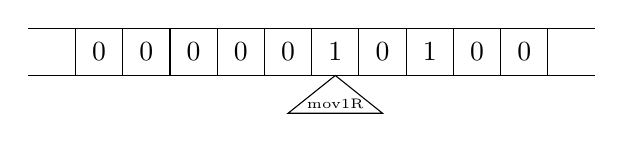
\begin{tikzpicture}[scale=0.6]
	\draw (0,0) -- (12,0);
	\draw (0,1) -- (12,1);
	\draw (1.5,0.5) node{0};
	\draw (2.5,0.5) node{0};
	\draw (3.5,0.5) node{0};
	\draw (4.5,0.5) node{0};
	\draw (5.5,0.5) node{0};
	\draw (6.5,0.5) node{1};
	\draw (7.5,0.5) node{0};
	\draw (8.5,0.5) node{1};
	\draw (9.5,0.5) node{0};
	\draw (10.5,0.5) node{0};
	\foreach \x in {1,...,11} \draw (\x,0) -- (\x,1);
	\draw (5.5, -0.8) -- (6.5, 0) -- (7.5, -0.8) -- cycle;
	\draw (6.5, -0.6) node{\tiny mov1R};
\end{tikzpicture}
\end{center}

\begin{center}
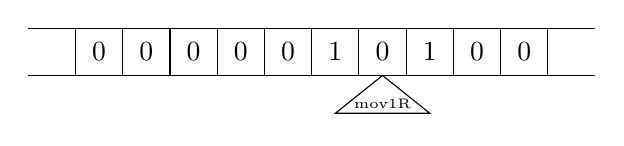
\begin{tikzpicture}[scale=0.6]
	\draw (0,0) -- (12,0);
	\draw (0,1) -- (12,1);
	\draw (1.5,0.5) node{0};
	\draw (2.5,0.5) node{0};
	\draw (3.5,0.5) node{0};
	\draw (4.5,0.5) node{0};
	\draw (5.5,0.5) node{0};
	\draw (6.5,0.5) node{1};
	\draw (7.5,0.5) node{0};
	\draw (8.5,0.5) node{1};
	\draw (9.5,0.5) node{0};
	\draw (10.5,0.5) node{0};
	\foreach \x in {1,...,11} \draw (\x,0) -- (\x,1);
	\draw (6.5, -0.8) -- (7.5, 0) -- (8.5, -0.8) -- cycle;
	\draw (7.5, -0.6) node{\tiny mov1R};
\end{tikzpicture}
\end{center}

\begin{center}
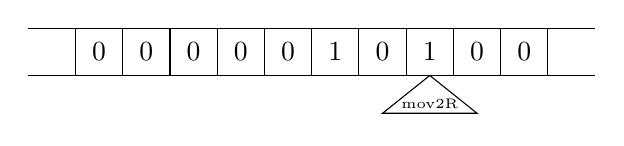
\begin{tikzpicture}[scale=0.6]
	\draw (0,0) -- (12,0);
	\draw (0,1) -- (12,1);
	\draw (1.5,0.5) node{0};
	\draw (2.5,0.5) node{0};
	\draw (3.5,0.5) node{0};
	\draw (4.5,0.5) node{0};
	\draw (5.5,0.5) node{0};
	\draw (6.5,0.5) node{1};
	\draw (7.5,0.5) node{0};
	\draw (8.5,0.5) node{1};
	\draw (9.5,0.5) node{0};
	\draw (10.5,0.5) node{0};
	\foreach \x in {1,...,11} \draw (\x,0) -- (\x,1);
	\draw (7.5, -0.8) -- (8.5, 0) -- (9.5, -0.8) -- cycle;
	\draw (8.5, -0.6) node{\tiny mov2R};
\end{tikzpicture}
\end{center}

\begin{center}
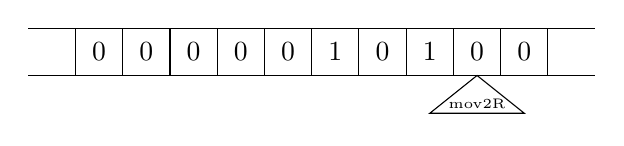
\begin{tikzpicture}[scale=0.6]
	\draw (0,0) -- (12,0);
	\draw (0,1) -- (12,1);
	\draw (1.5,0.5) node{0};
	\draw (2.5,0.5) node{0};
	\draw (3.5,0.5) node{0};
	\draw (4.5,0.5) node{0};
	\draw (5.5,0.5) node{0};
	\draw (6.5,0.5) node{1};
	\draw (7.5,0.5) node{0};
	\draw (8.5,0.5) node{1};
	\draw (9.5,0.5) node{0};
	\draw (10.5,0.5) node{0};
	\foreach \x in {1,...,11} \draw (\x,0) -- (\x,1);
	\draw (8.5, -0.8) -- (9.5, 0) -- (10.5, -0.8) -- cycle;
	\draw (9.5, -0.6) node{\tiny mov2R};
\end{tikzpicture}
\end{center}

\begin{center}
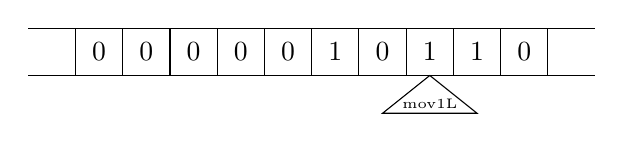
\begin{tikzpicture}[scale=0.6]
	\draw (0,0) -- (12,0);
	\draw (0,1) -- (12,1);
	\draw (1.5,0.5) node{0};
	\draw (2.5,0.5) node{0};
	\draw (3.5,0.5) node{0};
	\draw (4.5,0.5) node{0};
	\draw (5.5,0.5) node{0};
	\draw (6.5,0.5) node{1};
	\draw (7.5,0.5) node{0};
	\draw (8.5,0.5) node{1};
	\draw (9.5,0.5) node{1};
	\draw (10.5,0.5) node{0};
	\foreach \x in {1,...,11} \draw (\x,0) -- (\x,1);
	\draw (7.5, -0.8) -- (8.5, 0) -- (9.5, -0.8) -- cycle;
	\draw (8.5, -0.6) node{\tiny mov1L};
\end{tikzpicture}
\end{center}

\begin{center}
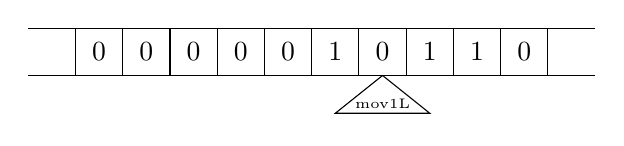
\begin{tikzpicture}[scale=0.6]
	\draw (0,0) -- (12,0);
	\draw (0,1) -- (12,1);
	\draw (1.5,0.5) node{0};
	\draw (2.5,0.5) node{0};
	\draw (3.5,0.5) node{0};
	\draw (4.5,0.5) node{0};
	\draw (5.5,0.5) node{0};
	\draw (6.5,0.5) node{1};
	\draw (7.5,0.5) node{0};
	\draw (8.5,0.5) node{1};
	\draw (9.5,0.5) node{1};
	\draw (10.5,0.5) node{0};
	\foreach \x in {1,...,11} \draw (\x,0) -- (\x,1);
	\draw (6.5, -0.8) -- (7.5, 0) -- (8.5, -0.8) -- cycle;
	\draw (7.5, -0.6) node{\tiny mov1L};
\end{tikzpicture}
\end{center}

\begin{center}
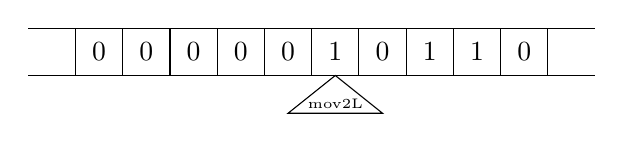
\begin{tikzpicture}[scale=0.6]
	\draw (0,0) -- (12,0);
	\draw (0,1) -- (12,1);
	\draw (1.5,0.5) node{0};
	\draw (2.5,0.5) node{0};
	\draw (3.5,0.5) node{0};
	\draw (4.5,0.5) node{0};
	\draw (5.5,0.5) node{0};
	\draw (6.5,0.5) node{1};
	\draw (7.5,0.5) node{0};
	\draw (8.5,0.5) node{1};
	\draw (9.5,0.5) node{1};
	\draw (10.5,0.5) node{0};
	\foreach \x in {1,...,11} \draw (\x,0) -- (\x,1);
	\draw (5.5, -0.8) -- (6.5, 0) -- (7.5, -0.8) -- cycle;
	\draw (6.5, -0.6) node{\tiny mov2L};
\end{tikzpicture}
\end{center}

\begin{center}
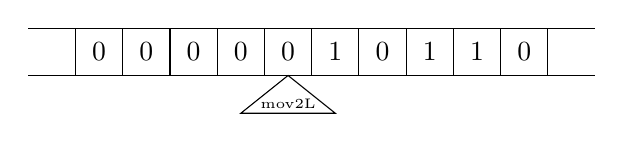
\begin{tikzpicture}[scale=0.6]
	\draw (0,0) -- (12,0);
	\draw (0,1) -- (12,1);
	\draw (1.5,0.5) node{0};
	\draw (2.5,0.5) node{0};
	\draw (3.5,0.5) node{0};
	\draw (4.5,0.5) node{0};
	\draw (5.5,0.5) node{0};
	\draw (6.5,0.5) node{1};
	\draw (7.5,0.5) node{0};
	\draw (8.5,0.5) node{1};
	\draw (9.5,0.5) node{1};
	\draw (10.5,0.5) node{0};
	\foreach \x in {1,...,11} \draw (\x,0) -- (\x,1);
	\draw (4.5, -0.8) -- (5.5, 0) -- (6.5, -0.8) -- cycle;
	\draw (5.5, -0.6) node{\tiny mov2L};
\end{tikzpicture}
\end{center}

\begin{center}
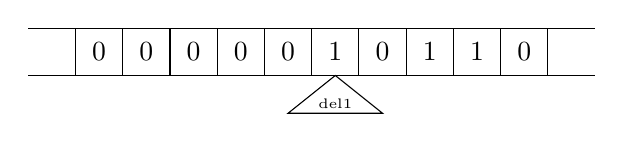
\begin{tikzpicture}[scale=0.6]
	\draw (0,0) -- (12,0);
	\draw (0,1) -- (12,1);
	\draw (1.5,0.5) node{0};
	\draw (2.5,0.5) node{0};
	\draw (3.5,0.5) node{0};
	\draw (4.5,0.5) node{0};
	\draw (5.5,0.5) node{0};
	\draw (6.5,0.5) node{1};
	\draw (7.5,0.5) node{0};
	\draw (8.5,0.5) node{1};
	\draw (9.5,0.5) node{1};
	\draw (10.5,0.5) node{0};
	\foreach \x in {1,...,11} \draw (\x,0) -- (\x,1);
	\draw (5.5, -0.8) -- (6.5, 0) -- (7.5, -0.8) -- cycle;
	\draw (6.5, -0.6) node{\tiny del1};
\end{tikzpicture}
\end{center}

\begin{center}
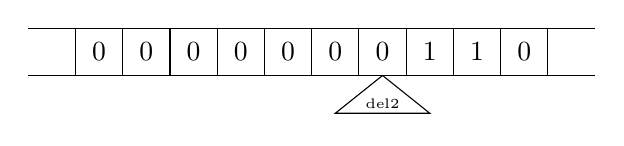
\begin{tikzpicture}[scale=0.6]
	\draw (0,0) -- (12,0);
	\draw (0,1) -- (12,1);
	\draw (1.5,0.5) node{0};
	\draw (2.5,0.5) node{0};
	\draw (3.5,0.5) node{0};
	\draw (4.5,0.5) node{0};
	\draw (5.5,0.5) node{0};
	\draw (6.5,0.5) node{0};
	\draw (7.5,0.5) node{0};
	\draw (8.5,0.5) node{1};
	\draw (9.5,0.5) node{1};
	\draw (10.5,0.5) node{0};
	\foreach \x in {1,...,11} \draw (\x,0) -- (\x,1);
	\draw (6.5, -0.8) -- (7.5, 0) -- (8.5, -0.8) -- cycle;
	\draw (7.5, -0.6) node{\tiny del2};
\end{tikzpicture}
\end{center}


\end{document}
